%------------------------------------------%
% Cannabis Data Science
% Saturday Morning Statistics
% 11/13/2021
%
% FIXME: Add bibliography
% https://tex.stackexchange.com/questions/148893/package-biblatex-error-incompatible-package-ucs-begindocument?noredirect=1&lq=1
% https://tex.stackexchange.com/questions/261595/how-to-rerun-biber-on-the-file
% https://tex.stackexchange.com/questions/229638/package-biblatex-warning-babel-polyglossia-detected-but-csquotes-missing
% https://tex.stackexchange.com/questions/49610/use-biblatex-and-utf8
% https://stackoverflow.com/questions/1507672/putting-citation-text-on-same-slide-with-latex-beamer
%------------------------------------------%
\documentclass[xcolor={dvipsnames}]{beamer}
\hypersetup{pdfpagemode=FullScreen}
\mode<presentation> %TEMPLATE
{ \usetheme{Boadilla}
  \usecolortheme{orchid}
  \usefonttheme{default}
  \setbeamertemplate{navigation symbols}{}
  \setbeamertemplate{caption}[numbered]} 
\usepackage[english]{babel}
\usepackage[utf8x]{inputenc}
\setbeamersize{text margin left=0.5in,text margin right=0.5in}

\usepackage[dvipsnames]{xcolor}
\definecolor{DarkGreen}{RGB}{2, 48, 32}
\definecolor{CalyxGreen}{RGB}{34, 153, 84}
\definecolor{DarkOrange}{RGB}{199, 0, 57}
\definecolor{LightOrange}{RGB}{255, 87, 51}
\definecolor{LightGreen}{RGB}{218, 247, 166}
\definecolor{LightYellow}{RGB}{255, 195, 0}

\setbeamercolor*{palette primary}{bg=LightGreen, fg = DarkGreen}
\setbeamercolor*{palette secondary}{bg=LightGreen, fg=DarkGreen}
\setbeamercolor*{palette tertiary}{bg=LightGreen, fg = DarkGreen}
%\setbeamercolor*{palette quaternary}{bg=myNewColorD, fg = green}

%------------------------------------------%
% FIXME: Bibliography
%------------------------------------------%
%\usepackage{csquotes}
%\usepackage[style=verbose]{biblatex}
%\addbibressource{presentation-bib.bib}

%------------------------------------------%
% Packages
%------------------------------------------%
\usepackage{amsmath}
\renewcommand*\footnoterule{} %No sperating line on footnote
\usepackage{mathtools} %ANNOTATING EQUATIONS
\usepackage{hhline} %DOUBLBARS
\usepackage[super]{nth}
\usepackage{graphicx, caption, subcaption}

%------------------------------------------%
% Commands
%------------------------------------------%
\newcommand\T{\rule{0pt}{2.5ex}} %TOPSTRUT
\newcommand\B{\rule[-1.25ex]{0pt}{0pt}} %BOTTOMSTRUT
\newenvironment<>{varblock}[2][.9\textwidth] %RESIZED BLOCKS
  {\setlength{\textwidth}{#1}
  \begin{actionenv}#3
    \def\insertblocktitle{#2}\par
    \usebeamertemplate{block begin}}
  {\par\usebeamertemplate{block end}
  \end{actionenv}}
\defbeamertemplate{enumerate item}{largeball} %LARGE BALLS
{\begin{pgfpicture}{-1ex}{-0.65ex}{1.5ex}{1.5ex}
\usebeamercolor[fg]{item projected}
{\pgftransformscale{2.5}\pgftext{\Large\pgfuseshading{bigsphere}}}
{\pgftransformshift{\pgfpoint{0pt}{0.5pt}}
\pgftext{\usebeamerfont*{item projected}\small\insertenumlabel}}
\end{pgfpicture}}
\usepackage{tikz} % FANCY ARROWS
\usepackage{xparse}
\NewDocumentCommand\UpArrow{O{2.0ex} O{black}}{%
   \mathrel{\tikz[baseline] \draw [->, line width=0.5pt, #2] (0,0) -- ++(0,#1);}} % FANCY UPARROW
\NewDocumentCommand\DownArrow{O{2.0ex} O{black}}{%
   \mathrel{\tikz[baseline] \draw [<-, line width=0.5pt, #2] (0,0) -- ++(0,#1);}} % FANCY DOWNARROW
%\vskip 1cm
\makeatletter
\newcommand{\LeftEqNo}{\let\veqno\@@leqno}%LEFT EQUATION #'s
\makeatother

%------------------------------------------%
% Title
%------------------------------------------%
\title[Saturday Morning Statistics]{}
\author{Cannabis Data Science}
\institute[]{\Large Saturday Morning Statistics}
\date{November \nth{13}, 2021}
\begin{document}
\begin{frame}{}
  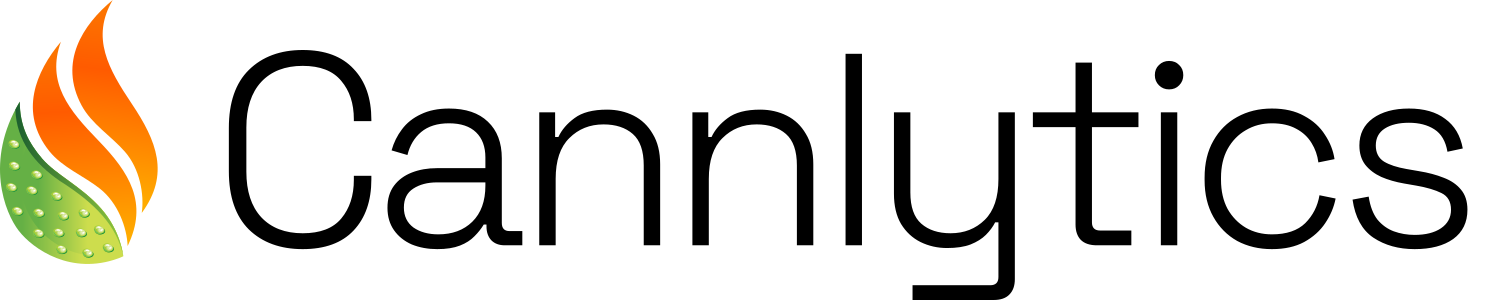
\includegraphics[scale=0.075]{images/logos/cannlytics_logo_with_text_light.png}
  \titlepage
\end{frame}

%------------------------------------------%
% Introduction
%------------------------------------------%

% TODO: Discuss Structural Breaks

% TODO: Discuss Difference-in-difference models

\section{Introduction}

\begin{frame}{}

\begin{figure}
    \begin{subfigure}[t]{0.6\textwidth}
      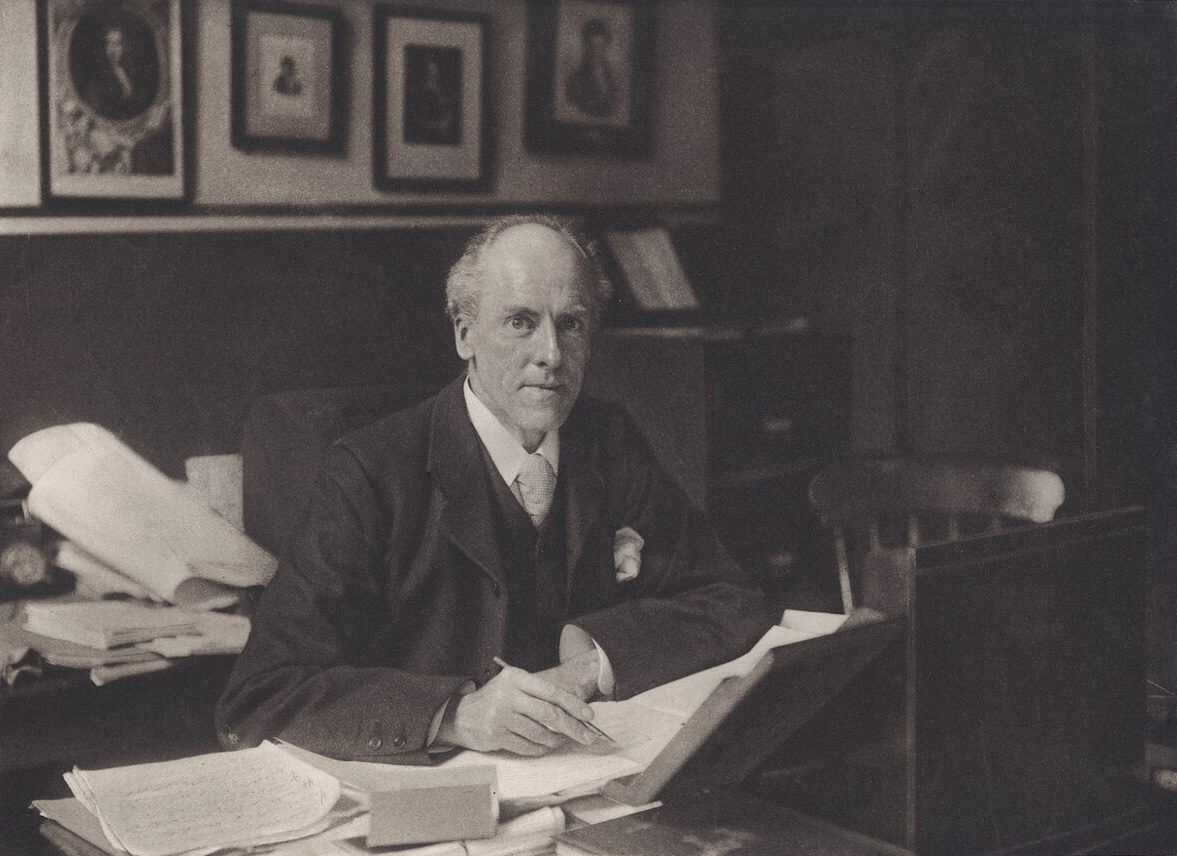
\includegraphics[width=\textwidth]{images/Karl_Pearson_1910.jpg}
    \end{subfigure}
    \caption*{Karl Pearson (1857 - 1936)}
\end{figure}

{\large Karl Pearson's contributions:}\vspace{0.25\baselineskip}\\

\begin{itemize}

\item Pearson correlation coefficient.

\item p-value.

\item Principal component analysis.

\item Created the first histogram.

\end{itemize}

\end{frame}


\begin{frame}{}

\begin{figure}
    \begin{subfigure}[t]{0.3\textwidth}
      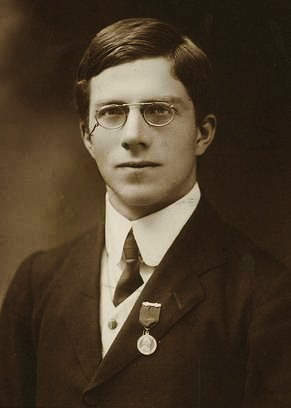
\includegraphics[width=\textwidth]{images/ronald-fisher.jpg}
    \end{subfigure}
    \caption*{Sir Ronald Fisher (1890 - 1962)}
\end{figure}

{\large Ronald Fisher's contributions:}\vspace{0.25\baselineskip}\\

\begin{itemize}

\item Introduced the term variance.

\item Analysis of variance (ANOVA).

\item Popularized the maximum likelihood estimation method.

\item The `F' of the F distribution is named in his honor.
\end{itemize}

\end{frame}


\section{Theory}


\begin{frame}{}

{\large Variance}\vspace{0.5\baselineskip}\\

\begin{figure}
    \begin{subfigure}[t]{0.6\textwidth}
      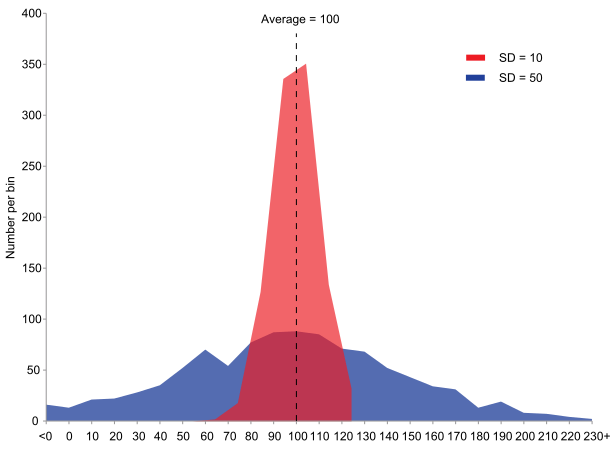
\includegraphics[width=\textwidth]{images/comparison_standard_deviations.png}
    \end{subfigure}
    \caption*{Example of samples from two populations with the same mean but different variances. The red population has mean 100 and variance 100 (SD=10) while the blue population has mean 100 and variance 2500 (SD=50).}
\end{figure}


\end{frame}


\begin{frame}{}
{\large Pearson Correlation Coefficient}\vspace{0.5\baselineskip}

\begin{figure}
    \caption*{Population correlation coefficient}
    \begin{subfigure}[t]{0.4\textwidth}
      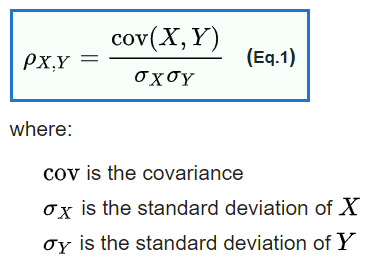
\includegraphics[width=\textwidth]{images/population_correlation_coefficient.png}
    \end{subfigure}
\end{figure}

\begin{figure}
    \caption*{Sample correlation coefficient}
    \begin{subfigure}[t]{0.6\textwidth}
      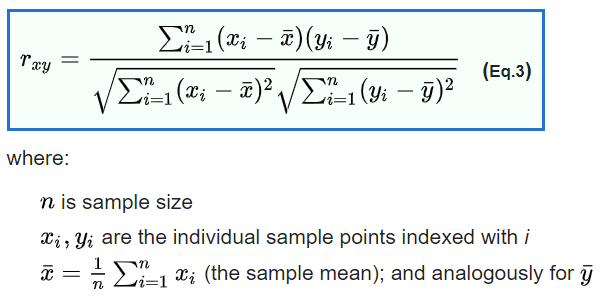
\includegraphics[width=\textwidth]{images/sample_correlation_coefficient.png}
    \end{subfigure}
\end{figure}

\end{frame}


\begin{frame}{}

\large{Analysis of variance (ANOVA)}\vspace{0.5\baselineskip}

\begin{itemize}

\item A statistical test of whether two or more population means are equal.

\item Generalizes the $t$-test beyond two means,

\end{itemize}

\begin{figure}
    \caption*{Hypothesis Test Type Errors}
    \begin{subfigure}[t]{0.6\textwidth}
      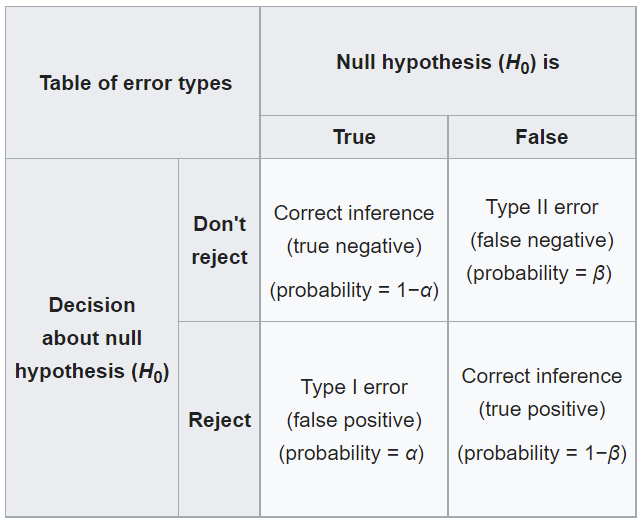
\includegraphics[width=\textwidth]{images/hypothesis_test_error_types.png}
    \end{subfigure}
\end{figure}

\end{frame}



\begin{frame}{}

{\large Modern Statistical Models}\vspace{0.5\baselineskip}\\

\begin{itemize}

\item \textbf{Fixed-effects models} - Apply to situations in which the experimenter applies one or more treatments to the subjects of the experiment to see whether the response variable values change. This allows the experimenter to estimate the ranges of response variable values that the \textit{treatment} would generate in the population as a whole.

\vspace{0.5\baselineskip}

\item \textbf{Random-effects models} - Used when the \underline{treatments are not fixed}. This occurs when the various factor levels are sampled from a larger population. Because the levels themselves are random variables, some assumptions and the method of contrasting the treatments differ from the fixed-effects model.

\end{itemize}

\end{frame}





\section{Application}

%------------------------------------------%
% Takeaway
%------------------------------------------%

\begin{frame}{}
\begin{center}
\begin{minipage}{3.85in}
Thank you for coming.
\end{minipage}
\end{center}
\end{frame}

%------------------------------------------%
\end{document}
%------------------------------------------%
